%% -*- coding: utf-8; -*-

% Use 'digital' option to enable back references. This option is recommended for digital pdf version
%\documentclass[phd,american,digital]{thesispuc}%english thesis
%\documentclass[mscr,american]{thesispuc}%english dissertation
%\documentclass[phd,brazilian]{thesispuc}%tese em portugês
\documentclass[msc,brazilian]{thesispuc}%disseretação em portuguŝ


%%%
%%% Additional Packages
%%%
\usepackage{tabularx}
\usepackage{multirow}
\usepackage{multicol}
\usepackage{colortbl}
\usepackage[%
    dvipsnames,
    svgnames,
    x11names,
    fixpdftex,
    table
]{xcolor}
\usepackage{numprint}
\usepackage{textcomp}
\usepackage{booktabs}
\usepackage{amsmath}
\usepackage{enumitem}
\usepackage{amssymb}
\usepackage{svg}
% ABNT reference style package. The current style is the alphabetical order, if you need
% change to citation order, change in the line above 'alf' to 'num', also at the end replace
% bibliographystyle with the commented version.
\usepackage[num]{abntex2cite}
%\usepackage{tikz}
%\usepackage[linesnumbered, ruled, vlined]{algorithm2e}
%\usepackage{pgfplots,pgfplotstable} 
%\usepackage{array}
\usepackage{longtable}


%% numprint 
\npthousandsep{.}
\npdecimalsign{,}

%% ThesisPUC option
%\tablesmode{fig} %% [nada, fig, tab ou figtab]
%\algoritmsmode{none} %% [none ou use] %% Default is [use]
%\codesmode{none} %% [none ou use] %% Default is [use]
%\abreviationsmode{none} %% [none ou use] %% Default is [use]

\tablesmode{figtab}

\algorithmsmode{none}
\codesmode{none}
\abreviationsmode{use}

% \makeatletter  \renewcommand\@biblabel[1]{#1}  \makeatother

%%%
%%% Counters
%%%

%% uncomment and change for other depth values
\setcounter{tocdepth}{1}
%\setcounter{lofdepth}{3}
%\setcounter{lotdepth}{3}
%\setcounter{secnumdepth}{3}

%%%
%%% Misc.
%%%

\usecolour{true}
%% \graphicspath{ {./figuras/} }
%% https://www.overleaf.com/learn/latex/Inserting_Images
\citebrackets[]

\renewcommand{\arraystretch}{1.5}


%%%
%%% Titulos
%%%

\tituloglossario{Lista de Abreviaturas}
\autor{Antenor Moreira de Barros Leal}
\autorR{Leal, Antenor Moreira de Barros}

\advisor{Adriano Francisco Branco}{Prof.}
\advisorR{Branco, Adriano Francisco}
% If the advisor's department is different from author's department, uncomment the next line and type the correct name and acronym of advisor's institution.
%\advisorInst{institution name}{acronym}

%\coadvisor{Otávio da Fonseca Martins Gomes}{Dr.}
%\coadvisorR{da Fonseca Martins Gomes, Otávio}
%\coadvisorInst{Centro de Tecnologia Mineral}{CETEM/MCTI}

\title{Aplicativo web de auxílio à navegação aérea}
\titleuk{Aerial navigation aid web application}

%%\subtitulo{Aqui vai o subtitulo caso precise}

\day{16}
\month{Junho}
\year{2024}

\city{Rio de Janeiro}
\CDD{004} 
\department{Informática}
\program{\mbox{Engenharia} da \mbox{Computação}}
\school{\mbox{Engenharia} da \mbox{Computação}}
\university{Pontifícia Universidade Católica do Rio de Janeiro}
\uni{PUC-Rio}


%%%
%%% Jury
%%%

\jury{%
  \jurymember{xxxxxxxxxxxxxxxx}{Prof.}
    {Departamento de Informática}{PUC-Rio}
  \jurymember{xxxxxxxxxxxxxxx}{Prof.}
    {Departamento de Informática}{PUC-Rio}
   \jurymember{xxxxxxxxxxxxxxx}{Prof.}
    {Departamento de Informática}{PUC-Rio}
}


%%%
%%% Personal Resume
%%%

\resume{%
% If it fit in one line use this command:
\makebox[\textwidth][s]{Graduando em Engenharia da Computação na PUC - Rio}%
% If not just type your resume without any special command 
}


%%%
%%% Catalog prekeywords
%%%

\catalogprekeywords{%
  \catalogprekey{Informática}%
}

%%%
%%% Keywords - Don't use % at the end of /key dfinition
%%%

\keywords{%
    \key{Aviação}
    \key{Navegação}
    \key{Aplicativo}
    \key{Algoritmo}
    \key{Web}
    \key{Internet}
}

\keywordsuk{%
    \key{Aviation}
    \key{Navigation}
    \key{Application}
    \key{Algoritm}
    \key{Web}
    \key{Internet}
}


%%%
%%% Abstract
%%%

\abstract{%
É um aplicativo web de código aberto com o objetivo de auxiliar usuários de simuladores de voo que não possuem
acesso à ferramenta (Electronic Flight Bag) que um piloto de linha aérea teria. Ao acessar o aplicativo, o usuário
se depara com a lista de aeroportos cadastrados e, após escolher um, são exibidas as informações da pista,
frequências do aeroporto (torre, solo, ATIS, etc.), e frequências de navegação (ILS, VOR, etc.). Também são
apresentadas as informações das condições meteorológicas atuais do aeródromo (vento, visibilidade,
temperatura, etc.), tanto no formato oficial (\abrev METAR), obtidas a cada hora de uma API externa, como em um texto
em linguagem natural para melhor entendimento do jogador iniciante. Um usuário com permissão de
administrador pode adicionar e editar aeroportos. Módulos adicionais estão disponíveis como o cálculo da pista
em uso (a partir de informações do vento) e do perfil de descida.
} 

\abstractuk{%
It is an open source web application to auxialiate the flight simulator's users that don't have
access to the tool (Electronic Flight Bag) that an airline pilot would have. When accessing the app, the users
encounter the list of registered airports and, after choosing one, runway information, airport frequencies 
(tower, ground, ATIS etc) and navigation frequencies (ILS, VOR etc) are showed. Also provided are the current 
meteorological conditions of the aerodrome (wind, visibility, temperature, etc.), both in the official 
format (METAR), obtained hourly from an external API, and in natural language text for better 
understanding by novice players. An administrator user can add and edit airports. Based on the 
current wind information, the active runway is calculated. Additional modules are available such as calculation 
of the runway in use (from wind information) and the descent profile.
}


%%%
%%% Dedication
%%%

% xxxxxxxxxxxxxxxxxxxxxxxx Dedicatória aqui xxxxxxxxxxxxxxxxxxxxxxx
\dedication{%
  
}

%%%
%%% Epigraph
%%%

% epígrafe xxxxxxxxxxxxxxxx
\epigraph{%
 
}
\epigraphauthor{ }
\epigraphbook{ }

%--------------------------------------------
% \usepackage{draftwatermark}

% \SetWatermarkText{{\normalfont SEGUNDA ENTREGA (26/06) rev 1}}

% \SetWatermarkScale{0.2}
% \SetWatermarkAngle{0}
% \SetWatermarkColor{red!80!white}
% \SetWatermarkHorCenter{0.5\paperwidth}
% \SetWatermarkVerCenter{0.1\paperheight}
%--------------------------------------------


\begin{document}
  \chapter{Introdução}
Com o aumento da capacidade de passageiros e carga e a necessidade 
de uma maior segurança, começou a se fazer necessário trazer ao cockpit 
vários documentos como checklist de procedimentos; log book; cartas de 
navegação, de saída, de aproximação, do aeródromo; tabelas de performance
 da aeronave etc.

Para levar tudo isto costumava-se usar uma maleta (a Flight Bag), 
obviamente esta ficava muito pesada.

Com a miniaturização dos computadores e surgimento dos tablets, 
começaram a ser desenvolvidos programas que substituem partes ou 
todos estes documentos, é a chamada maleta de voo eletrônica, mais 
conhecida pela sigla em Inglês EFB (\textit{Electronic Flight Bag}).

Atualmente existem hardwares dedicados para esta função, mas é mais 
comum se usar um tablet com um aplicativo disponibilizado pela companhia aérea.
Normalmente, o tablet escolhido é um iPad da Apple, mas algumas companhias
optaram pelo Microsoft Surface. \cite{surface}

O uso do EFB trouxe uma série de benefícios para os pilotos e para as 
companhias aéreas. Além de reduzir o peso e o volume de documentos físicos 
a serem transportados, o EFB permite uma rápida atualização das informações, 
garantindo que os pilotos tenham sempre acesso às versões mais recentes das 
cartas de navegação. \cite{EFB-more-than}

Além disso, a capacidade de armazenamento do EFB possibilita o acesso a uma 
vasta quantidade de informações adicionais, como manuais de operação da aeronave, 
regulamentações atualizadas e até mesmo dados meteorológicos em tempo real, 
o que contribui para uma tomada de decisão mais informada e segura durante o voo.

  \chapter{Situação atual}
Com o aumento da capacidade de passageiros e carga e a 
necessidade de uma maior 
segurança, começou a se fazer necessário trazer ao cockpit vários
documentos como checklist de procedimentos; log book; cartas de 
nevagação, de saída, de aproximação, do aerodromo; tabelas de 
performance da aeronave etc. 

Para levar tudo isto costumava-se usar uma maleta (a Flight Bag),
obviamente esta ficava muito pesada.

Com a minituarização dos computadores e surgimentos os tablets, 
comecaram a ser desenvolvidos programas que subsituiam partes
ou todos estes documentos, é a chamada maleta de voo eletrônica,
mais conhecida pela sigla em Inglês EFB (Electronic Flight Bag).

Nos simuladores de voo para computador pessoal, algumas aeronaves
simulam este equipamento como o Airbus A320neo desenvolvido pela
FlyByWire Simulations. Apesar de ser uma aeronave freeware, ela 
é bem sofisticada chegando ao nível de realismo da Fenix Simulations
ou da ToLiss Simulations, duas produtoras com modelos pagos do A320.

\begin{figure}[ht]
    \begin{center}
    \includegraphics[width=400pt]{img/efb-a320.png}
    \caption{Exemplo de um EFB no Flight Simulator 2020 na aeronave A320neo}
    \label{fig:efb-a320}
    \end{center}
\end{figure}

Contudo, o METAR do aeródromo não se encontra disponível no EFB.
É possível usar o computador de bordo da aeronave (FMC) e conseguir
esta informação. Também é possível sintonizar na frequência do ATIS,
mas isto só funcionará se o avião já estiver perto de aeródromo.

O que muitos jogadores fazem é acessar o AISWEB, sistema oficial brasileiro
de informações aeronáuticas. 

\begin{figure}[ht]
    \begin{center}
    \includegraphics[width=400pt]{img/aisweb.png}
    \caption{AISWEB com informações de pista frequências de comunicação e navegação para o Santos Dumont}
    \label{fig:aisweb}
    \end{center}
\end{figure}

É um site extremamente completo, podendo
ser usado em operações reais, mas para o jogador iniciante seria 
de valia uma interface mais simples.
  \chapter{A Proposta}
A ideia do trabalho é unir as funcionalidades do METAR-TAF com o AISWEB
em uma aplicação web que o usuário iniciante consiga usar sem dificuldades.

Pelo fato de aviação necessitar ter um ambiente seguro e bastante regulado, considerando
que meu projeto é apenas um protótipo, prefiro restringir o caso de uso apenas
para jogadores de simuladores de voo que desejam que a simulação seja parecida
com o real. Nas páginas do sistema conterá um aviso de que o sistema \textbf{"não
deve ser usado para um voo real"}.

Dito isto, o sistema possui backend escrito na linguagem Python, fazendo uso da 
framework FastAPI. Até a entrega do Projeto I, o backend era feito com Flask. 
A escolha foi feita pela minha familiaridade com a framework. Porém, depois, 
descobri a framework FastAPI no meu trabalho. Normalmente, ela não é usada para fullstack, mas 
sim para fazer APIs REST, que retornam JSON na resposta de uma requisição. Um 
frontend feito em alguma framework de JavaScript faria a requisição e atualizaria a página
a partir dos dados recebidos.

Contudo, é possível retornar qualquer tipo de dado no FastAPI, inclusive páginas HTML. 
Como prefiro fazer a renderização de páginas no lado do servidor, continuei usando 
a funcionalidade de templates do Jinja2.

A substituição da framework deu-se pelos seguintes motivos:

\begin{itemize}
\item Projeto mais maduro, continuamente mantido.
\item Documentação bem mais detalhada do que a do Flask, com vários tutoriais sobre assuntos comumente usados, como autenticação e sessão de usuário.
\item Servidor embutido (Uvicorn) extremamente fácil de configurar e suficiente para produção \cite{fast-api-prod}.
No Flask é necessário configurar alguns parâmtros para o Guinicorn via o arquivo "gunicorn\_config.py".
\item Assíncrono, permitindo o uso junto com bibliotecas que utilizam asyncio.
No Flask, para paralelismo, é necessário usar uma biblioteca como o Gevent.
\end{itemize}

No segundo semestre de 2023 comecei a fazer este projeto para uso próprio.
O código está disponível em \url{https://github.com/antenor-z/aero}. Atualmente o
projeto funciona, mas a arquitetura foi feita sem muito planejamento, as
informações do aeroporto são hardcoded.

O usuário tem acesso a informações de frequência da torre, solo, tráfego, rampa
e operações, bem como das frequências e dados para VOR (um sistema de radionavegação
por antenas no solo), ILS (sistema de pouso por instrumentos) e informações
de pista. Neste trabalho quero, armazenar estas
em um banco de dados relacional com uma arquitetura bem planejada. Farei testes
de desempenho simulando uma alta taxa de acesso e, dependendo dos resultados,
fazer uso de um banco em memória como intermediário. 

Os aeródromos podem, ao longo do tempo, mudarem alguma frequência e outras
informações, como o número da pista, que muda a depender da variação do norte magnético,
uma ampliação da pista faz a informação de comprimento precisar ser alterada...

O código precisava ser alterado para atualizar estas informações.
É implementado um sistema administrativo no site, com uma autenticação por
senha e TOTP, para que seja possível mudar qualquer informação no banco mesmo
por pessoas que não saibam programar.

Esta parte administrativa, possui controle de permissões. Ao criar uma
conta, eu informo quais aeroportos esta conta pode alterar. Também posso
dizer que esta é uma conta "super" que pode alterar todos os aeroportos
e também criar e apagar um aeroporto.

Através de uma API do serviço americano National Weather Service, são coletadas 
as informações atuais de meteorologia. Estas informações (que vêm em um formato
chamado METAR) são processadas pelo backend e mostradas ao usuário de uma forma 
fácil de entender. Esta parte em específico possuia um código de difícil manutenção.
Foi refatorada esta parte e adicionado suporte para a maior parte de códigos
da especificação do METAR.

Ao longo do tempo, acessava o site, e caso visse alguma parte do METAR sem explicação,
adicionava no algorítmo. Atualmente todas as informações são explicadas para
os aeródromos brasileiros. Mais informações no capítulo de "Decodificação do METAR".

  % Revisão OK 25/09
\chapter{Princípios norteadores}

Para este projeto segui os seguintes princípios por ordem de prioridade começando
pela maior prioridade.

\section{Exatidão da Informação Apresentada}
Não devem haver erros na explicação do METAR, TAF e nas informações do aeródromo. 
Claro que não é possível aderir a este princípio em 100\% dos casos, pois uma 
informação de aeroporto pode mudar. No entanto, comparo constantemente minhas 
informações com o AISWeb e, em caso de alterações, é possível fazê-las facilmente
pela área restrita do site.

\section{Rapidez no Carregamento das Páginas} Nenhum arquivo externo como .js, 
.css, .ttf, etc., é coletado externamente. Os arquivos estáticos estão no servidor. 
A geração das páginas inclusive dos gráficos é feita no lado do servidor. O que 
precisa rodar no lado do cliente, como pesquisas e tooltips, é implementado com 
JavaScript puro.

Os gráficos com informações históricas são construídos de forma assíncrona, e os
dados de METAR e TAF são coletados da API do Aviation Weather e inseridos no
banco de dados também de forma assíncrona. Assim, quando o usuário carrega a 
página, essas informações já estão prontas para o envio.

Como será visto no capítulo de arquitetura existe uma proxy reversa com NGINX,
esta proxy faz cache das páginas, então se uma página é recarregada muitas vezes
seguidas o NGINX entrega a página salva no cache. O cache está configurado para
ser invalidado em um minuto, então, no pior caso, as informações ficam com um 
minuto de atraso. A informação que atualiza com mais frequência é o METAR. A
atualização ocorre de hora em hora, então o atraso de um minuto, no máximo, é
aceitável.

\section{Facilidade de Uso do Sistema} A diagramação das páginas é feita
considerando que o usuário pode não ter um conhecimento avançado em aviação, mas
deseja acessar todas as informações de um aeródromo. Essas informações estão 
divididas em três páginas para cada aeródromo, para que a visualização não fique 
sobrecarregada.
  % Revisão OK 30/09
\chapter{Cronograma}

Para ter uma direção do projeto e medição da evolução, ele foi dividido em várias 
tarefas com início e duração esquematizados abaixo.

O que está em laranja são grupos de tarefas, em preto são as tarefas em si, as 
células com fundo em azul são a(s) semana(s) planejadas para realizar cada tarefa. 
O símbolo de losango mostra quando a tarefa foi de fato feita.

Em vermelho, temos tarefas que não estavam no planejamento.

\section{Cronograma do Projeto Final I}

\begin{figure}[ht]
    \begin{center}
    \includesvg[width=\linewidth]{img/cronograma.svg}
    \caption{Cronograma I}
    \label{fig:cronograma-planejado-I}
    \end{center}
\end{figure}

Os dias 29/05 e 26/06 são milestones onde ocorrem as entregas.

\begin{table}[h]
    \centering
    \caption{Milestones}
    \begin{tabular}{|c|l|}
        \hline
        \textbf{Data} & \textbf{Milestone} \\
        \hline
        29/05 & Entrega da proposta de Projeto Final I \\
        26/06 & Entrega do relatório de Projeto Final I \\
        \hline
    \end{tabular}
\end{table}

Por ter sido meu primeiro grande projeto autogerido, tive um pouco de dificuldade 
em estimar o tempo real de implementação de cada tarefa. Portanto, há uma grande 
diferença entre quando uma tarefa foi estimada para ser feita e quando ela realmente 
o foi.

As seguintes tarefas são propostas para a segunda parte do projeto.

\begin{itemize}
    \item Usuários autenticados alterarem informações de um aeroporto;
    \item Cálculo das componentes do vento;
    \item Cálculo do perfil de descida;
    \item Geração de gráficos históricos para um aeroporto;
    \item Visualização das posições dos aeroportos em um mapa.
\end{itemize}

\section{Cronograma do Projeto Final II}

\begin{figure}[ht]
    \begin{center}
    \includesvg[width=\linewidth]{img/cronograma2.svg}
    \caption{Cronograma II}
    \label{fig:cronograma-planejado-II}
    \end{center}
\end{figure}

\begin{table}[h]
    \centering
    \caption{Milestones}
    \begin{tabular}{|c|l|}
        \hline
        \textbf{Data} & \textbf{Milestone} \\
        \hline
        06/09 & Entrega do formulário de Projeto Final II \\
        15/11 & Entrega do Projeto Final II \\
        25/11 a 29/11 & Bancas Projeto Final II \\
        \hline
    \end{tabular}
\end{table}
  \chapter{Decodificação do METAR}

\section{Introdução}
O METAR é um protocolo de transmissão de dados meteorológicos de um aeroporto ou aeródromo. Não se trata de 
uma previsão do tempo, mas sim de uma visualização atual. O METAR é formado por itens separados por espaço. 
Cada item corresponde a uma unidade mínima de informação meteorológica. Com os dados de sensores instalados 
no aeródromo \cite{metar-weather-gov}, a cada hora é publicado um novo METAR que é válido para aquela hora. 
Em casos excepcionais, quando as condições de tempo estiverem mudando repentinamente, um METAR pode ser atualizado 
a cada meia hora \cite{METAR-speci}.

\section{Exemplo}
O METAR no aeroporto de Fortaleza \cite{METAR-sbfz}, no dia 17 de abril de 2024 às 10:54 foi
\texttt{171300Z 15010KT 9999 BKN019 SCT025 FEW030TCU BKN100 30/25 Q1011}.

"SBFZ" se refere ao código ICAO (International Civil Aviation Organization) do aeroporto, não confundir 
com o código IATA (International Air Transport Association) que é formado por três letras. O aeroporto Pinto 
Martins possui o código IATA FOR, o Santos Dumont SDU e o Galeão GIG. O público geral parece conhecer mais este 
código, mas na aviação costuma-se usar mais o código ICAO, pois \textit{todos} os aeródromos possuem um, 
enquanto o IATA só é presente em aeroportos onde há processamento de bagagem \cite{iata-codes} \cite{icao-codes}.

O ICAO é formado por quatro letras em que a primeira é o prefixo da região. A América do Sul possui o prefixo "S", 
o Brasil possui o prefixo "SB", por isso que os aeroporto de Fortaleza, Santos Dumont e Galeão possuem os códigos 
SBFZ, SBRJ e SBGL, respectivamente. Países com muitos aeroportos, apenas uma letra, 
logo as três últimas letras ficam livres, podendo assim ter mais códigos para uso.

\texttt{171300Z} significa que este METAR se refere ao dia 17 às 13 horas e zero minuto zulu. Horário zulu é 
simplesmente o fuso horário da longitude de zero grau, chamado de hora UTC ou Coordinated Universal Time \cite{UTC}. 
Para que não haja confusão com os horários, a aviação internacionalmente usa o horário UTC. Este METAR será 
válido até às 13:59, quando será substituído pelo METAR iniciando com "SBFZ 171400Z".

Note que a seguinte expressão regular com três grupos de captura consegue extrair o dia, a hora e o minuto:

\begin{verbatim}
([0-9]{2})([0-9]{2})([0-9]{2})Z
\end{verbatim}

Com o METAR supracitado, os grupos de captura serão:

\begin{itemize}
\item Grupo 1 (dia): 17
\item Grupo 2 (hora): 13
\item Grupo 3 (minuto): 00
\end{itemize}

\texttt{15010KT} se refere à velocidade e direção do vento. Os três primeiros algarismos informam a direção, 
em graus, de onde o vento sopra, e os últimos dois algarismos informam a velocidade do vento em nós (milhas náuticas por hora). 
Neste caso, o vento vem da direção 150 graus com velocidade de dez nós. Com a expressão abaixo extraímos essas duas informações:

\begin{verbatim}
([0-9]{3})([0-9]{2})KT
\end{verbatim}

A informação de vento pode também conter a letra G (gust) para rajadas e a letra V em um item separado para o 
caso de haver variação de direção. Por exemplo, um METAR com os itens \texttt{10016G21KT 080V120} informa que 
há rajadas de até 21 kt e a direção do vento pode variar de 80 a 120 graus. Existem outros aeroportos que podem 
usar outras unidades para a velocidade do vento, mas no Brasil só é usado nós (kt). Para obter essas informações 
usamos o regex \texttt{([0-9]{3}[0-9]{2}G{[0-9]{2}})} e \texttt{([0-9]{3})V([0-9]{3})}.

\texttt{9999} significa visibilidade ilimitada (maior ou igual a 10 km). Se fosse 6000, a visibilidade seria de 
6 km. Por ser sempre quatro algarismos, o regex \texttt{([0-9]{4})} consegue capturar essa informação.

\texttt{30/25} Temperatura 30°C e ponto de orvalho 25°C. Caso a temperatura seja negativa, a letra M é adicionada 
antes do número. M2/M5 significa temperatura -2°C e ponto de orvalho -5°C \cite{METAR-help}.

\texttt{Q1012} O altímetro do avião deve ser referenciado para 1012 hectopascal. Também pode ser usada a unidade 
polegadas de mercúrio (mmHg), mas no Brasil esta não é usada no METAR.

\texttt{SCT025} Nuvens espalhadas (3/8 a 4/8 do céu com nuvens) em 2500 pés de altitude. 025 se refere ao nível 
de voo (Flight Level), que é a altitude acima do nível médio do mar com divisão exata por 100.

\texttt{FEW030TCU} Poucas nuvens (1/8 a 2/8 do céu com nuvens) em 3000 pés de altitude. O sufixo TCU significa 
que há nuvens convectivas significativas \cite{decea-mil}.

\texttt{BKN100} Nuvens broken (5/8 a 7/8 do céu com nuvens) em 10000 pés de altitude.

Existe também o tipo OVC (overcast) que se refere a totalmente encoberto.

\section{Algoritmo}

O objetivo do módulo de decoder é dar uma explicação semelhante a esta para qualquer tipo de METAR de aeroportos 
no Brasil. O módulo usa várias expressões regulares para decodificar uma grande quantidade de informações, porém 
não é exaustivo; foi dada preferência a fenômenos que podem ocorrer no Brasil \cite{decea-mil}.

O algoritmo deve separar a string do METAR pelo caractere de espaço. Para cada item separado, cada expressão regular 
é testada. Caso uma combinação ocorra, os grupos de captura são interpolados em uma string que explica aquele item. 

Semdo "\$1" o primeiro grupo de captura e "\$2" o segundo, se o item "27008G16KT" é encontrado pela expressão 
\begin{verbatim}
  ([0-9]\{3\})([0-9]\{2\})G([0-9]\{2\})KT
\end{verbatim}

o algorítmo interpola a frase:

\begin{verbatim}
  Vento \$1° com \$2 nós e rajadas de até \$3 nós
\end{verbatim}

com os grupos de captura do regex supracitado. Então será gerada uma tupla
\texttt{(27008G16KT, Vento 270° com 8 nós e rajadas de até 16 nós)}. O retorno do 
algorítmo será uma lista de tuplas que será enviada a ferramenta de templating
de página Jinja.

\section{Complexidade Temporal}
Considerando que todas as expressões usadas são simples, isto é, não levam a backtracking, 
a complexidade temporal para executar a função \texttt{re.findall()} do Python é

$$ O_{findall}(m + n) $$

\begin{verbatim}
m := quantidade de caracteres da expressão regex
n := quantidade de caracteres da string a ser analisada
\end{verbatim}

Se temos que testar todas as expressões para cada item do METAR, a complexidade será

$$ O_{decode}(p * q * (m + n)) $$

\begin{verbatim}
m := quantidade de caracteres da expressão regex
n := quantidade de caracteres da string do METAR a ser analisado
p := quantidade de itens do METAR
q := quantidade de expressões regex no programa
\end{verbatim}


A maior expressão regex no decoder é \texttt{([A-Z]{3})(\d{3})(CB|TCU)*} com 26 caracteres.
Para efeitos práticos este é um valor muito pequeno então podemos assumir m constante.

Sabemos que o número de expressões é 11, também um valor que pode ser assumindo contante, logo
q é igual à 1, portanto.

$$ O_{decode}(p * 1 * (1 + n)) $$
$$ O_{decode}(p * n) $$

Apenas as variáveis "p" e "n" dependem de valores externos. 

  \chapter{Decodificação do TAF}

O TAF (\textit{Terminal Aerodrome Forecast}) é um protocolo que fornece
previsões para aeroportos. Diferente
do METAR, que relata as condições meteorológicas atuais, o TAF projeta o que se
espera para as próximas horas e/ou dias. Uma diferença em relação ao METAR é que o 
TAF se entende por várias linhas.
A partir da segunda linha, temos os chamados grupos temporais. Tudo que está em uma linha
são condições que irão ocorrer dentro de uma faixa de tempo. 

Um grupo temporal pode começar com BECMG ou TEMPO.

\begin{enumerate}
\item BECMG: Indica uma mudança gradual e definitiva nas condições meteorológicas;
\item TEMPO: Indica uma mudança temporária nas condições.
\end{enumerate}


Neste capítulo, será apresentado um exemplo de TAF, sua decodificação,
e uma explicação do algoritmo utilizado.

\section{Exemplo}
O TAF emitido para o aeroporto de Pinto Martins (SBFZ) no dia 31 de agosto 
de 2024 às 09:00Z foi:

\begin{verbatim}
310900Z 3112/0112 15010KT CAVOK TX31/3115Z TN24/0108Z 
  BECMG 3115/3117 11015KT FEW025 
  BECMG 0104/0106 15010KT RMK PHD
\end{verbatim}

\texttt{310900Z} significa que este TAF foi gerado dia 31 às 09:00 UTC. 3112/0112 indica 
o período válido desta informação: do dia 31 às 
12 horas até dia primeiro às 12 horas. 15010KT indica um vento de 10 nós vindo 
da direção 150 graus. Não há nuvens e a visualidade é máxima. É usado o acrônimo 
CAVOK (Ceiling Altitude and Visibility OK, Teto e Visibilidade OK) para indicar isto.

\texttt{TX31/3115Z TN24/0108Z} A temperatura mínima será de 24 graus dia 01 às 08:00 (UTC) e a máxima será 
de 31 graus no dia 31 as 15:00 (UTC).

A seguir, vêm os grupos de previsão, cada um em uma linha.

\texttt{BECMG 3115/3117 11015KT FEW025}: Dia 31 das 15 às 17 horas UTC terá vento de 
15 nós com 110 graus. E haverá poucas nuvens na altitude no nível 025 ou 2500 pés.

\texttt{BECMG 0104/0106 15010KT RMK PHD} : dia primeiro de setembro das 04:00 as 06:00, 
o vento será de 10 nós com 150 graus.

RMK adiciona uma observação (remark). O trigrama PHD representa a identificação 
do previsor que gerou este TAF. É algo específico do Brasil [16].

É claro que há muitos outros itens possíveis dentro da especificação. PROB30 em 
um grupo de previsão, por exemplo, informa que as informações nesta linha tem 
30\% de chance de ocorrer.

O objetivo do decodificador é explicar corretamente qualquer TAF brasileiro.


\section{Algoritmo}

O algoritmo para lidar com um TAF é semelhante ao utilizado para o METAR, porém adaptado
para as especificidades das previsões temporais. O TAF é segmentado em diversas
partes, cada uma sendo processada individualmente por expressões regulares para extrair as
informações relevantes.

Para cada item do TAF, o algoritmo tenta associar a string correspondente a uma descrição
detalhada utilizando expressões regulares pré-definidas. Por exemplo, a expressão

\begin{verbatim}
[0-9]{4}/[0-9]{4} 
\end{verbatim}

é usada para identificar os períodos de tempo, enquanto a expressão

\begin{verbatim}
[0-9]{3}([0-9]{2})KT
\end{verbatim}

é utilizada para extrair a direção e velocidade do vento.

Assim como no METAR, as informações são organizadas em tuplas que contêm a string original
e sua decodificação correspondente. Essas tuplas são então enviadas para um sistema de
templating \textit{Jinja2}, para a geração da página HTML.

\section{Exemplo de Resposta}

\lstinputlisting[label=rett:taf, language=Python]{code/taf.json}

  % \input{chapters/5-vento}
  % Revisão OK 12/10
\chapter{Modelo de Dados}

Nesta seção, explica-se o modelo de dados desenvolvido para o projeto, abordando 
sua estrutura lógica e os componentes principais. O objetivo deste modelo é garantir 
flexibilidade para futuras alterações e manutenções, proporcionando uma base sólida 
e expansível para o projeto.

\section{Modelo Lógico}

O modelo de dados foi feito de forma que futuras alterações possam ser absorvidas 
facilmente. Abaixo está o diagrama entidade-relacionamento, no qual o nome no topo 
do retângulo identifica o nome da tabela. A lista abaixo do nome mostra as colunas 
dessas tabelas, a sigla PK denota \textit{chave primária} e FK \textit{chave estrangeira}.

Uma relação é denotada pelas setas ligando duas tabelas. A cardinalidade da relação é indicada
pelos números entre parênteses. 

Para a relação \texttt{Aerodrome-ILS}, temos (1, 1) para (0, n), significando que 
um aeródromo pode ter zero ou mais frequências de ILS e esta só pode ser de um único 
aeródromo.

Já na relação \texttt{Aerodrome} com \texttt{Runway}, um aeródromo deve ter \texttt{uma ou mais} pistas
e uma pista pertence a um único aeródromo.

\pagebreak

\begin{figure}[ht]
    \begin{center}
    \includegraphics[width=400pt]{img/ERAero.png}
    \caption{Diagrama lógico}
    \label{fig:diagrama-er}
    \end{center}
\end{figure}

Note-se que as tabelas "CommunicationType", "ILSCategory" e "PavementType" poderiam 
ser substituídas por colunas enum nas tabelas "Communication", "ILS" e "Runway", 
porém a manutenção seria difícil \cite{table-enum}, pois teríamos que alterar a 
estrutura das tabelas (possivelmente tirando o Aero do ar) caso fosse necessário 
adicionar um tipo novo de comunicação, por exemplo. Fazendo com uma tabela externa 
é necessário apenas adicionar uma nova linha.

\section{Noções sobre o Funcionamento de um Aeródromo}

Antes de discutir as tabelas, é interessante compreender algumas regras e 
características básicas do funcionamento de um aeródromo. Isto certamente
facilitará o entendimento das colunas das tabelas.

Um aeródromo é a área destinada às operações de pouso, decolagem, e taxiamento 
de aeronaves, abrangendo pátio, taxiways (vias de taxi) e pistas. O terminal de 
passageiros, no entanto, não faz parte do aeródromo em si. Por isso, todos os 
aeroportos são aeródromos, mas nem todo aeródromo é um aeroporto, pois nem todos 
possuem infraestrutura para o atendimento de passageiros.

\subsection{Pistas}

Para o entendimento do funcionamento das pistas de pouso e decolagem, é importante 
conhecer algumas de suas características essenciais, como comprimento e largura, 
que impactam diretamente as operações das aeronaves.

O comprimento da pista, por exemplo, influencia a quantidade de frenagem necessária 
para uma aeronave parar com segurança após o pouso. Em pistas curtas, certos 
modelos de aeronaves não podem pousar com segurança. Já a largura da pista limita 
a envergadura máxima das aeronaves que podem operar nela. Em pistas muito estreitas, 
uma aeronave de grande porte, como o Boeing 747, pode ter dificuldades adicionais: 
os motores mais externos podem ultrapassar a área pavimentada, expondo-os a 
materiais no gramado, o que aumenta o risco de ingestão de objetos.

No caso de cabeceiras paralelas, ou seja, pistas que apontam para a mesma direção, 
temos as seguintes configurações:

\subsubsection{Pista Única}

A numeração da cabeceira da pista é determinada pela sua orientação magnética, 
dividida por 10 e arredondada. Por exemplo, em Fortaleza, a cabeceira com 
orientação de 126 graus é numerada como 13 (126 dividido por 10 é igual a 
12,6, que arredondamos para 13).

\subsubsection{Pista Dupla}

Para pistas paralelas duplas, são usadas as letras "L" (Left, esquerda) e "R" 
(Right, direita) para distinguir as cabeceiras. No aeroporto Santos Dumont, por 
exemplo, temos as cabeceiras 02L (esquerda) e 02R (direita), quando o observador 
está de costas para o Pão de Açúcar.

\subsubsection{Pista Tripla}

Embora no Brasil não haja aeroportos com três pistas paralelas, em outros países, 
onde existem pistas triplas, são utilizadas as letras "L" (left/esquerda), "C" 
(center/central) e "R" (right/direita) para identificação das cabeceiras.

\subsection{Comunicação}

As frequências de comunicação em aeródromos utilizam modulação de amplitude (AM), com banda 
de 118 MHz a 137 MHz. Cada aeródromo possui frequências específicas para cada fase 
do voo, como autorização, taxi, decolagem, aproximação e pouso.

Os tipos de frequência achadas em aeroportos do Brasil são:

\begin{enumerate}
\item Tráfego
\item Torre
\item Solo
\item Rampa
\item ATIS
\item Operações
\end{enumerate}

Nesta trabalho, para cada aeroporto, são mostradas as frequencias usadas com seus
tipos.

\subsection{Navegação}

As frequências de navegação são utilizadas pelos sistemas de localização do avião, 
não transmitindo áudio, mas sim dados, dentro da faixa de 108 a 117.95 MHz. Esses 
sistemas ajudam a determinar a posição e a trajetória da aeronave com precisão.

\begin{itemize} 
\item VOR (Very High Frequency Omnidirectional Range): Um sistema 
de navegação baseado em uma antena no solo, o VOR permite que a aeronave 
determine a direção que deve seguir para passar diretamente sobre a antena, 
indicando essa direção em um instrumento específico na cabine. Na aviação isto
é chamado de bloqueio de VOR. \cite{vor-block}

\item ILS (Instrument Landing System): Sistema de aterrissagem por instrumentos 
que transmite informações de orientação lateral (alinhamento com o eixo da pista) 
e orientação vertical (ângulo de descida) específicas para cada cabeceira da pista. 
Essas informações permitem uma aproximação precisa, mesmo em condições de baixa 
ou nenhuma
visibilidade. O ILS pode ser usado tanto para pouso manual, onde o piloto controla
a aeronave seguindo 
as indicações, quanto para pouso automático (auto land), caso a aeronave possua 
esta capacidade. \cite{ils-train}
\end{itemize}

Neste trabalho são mostradas as frequências de ILS e VOR para cada aeroporto.

\section{Dicionário de Dados}

\begin{longtable}{|p{3.2cm}|p{6.4cm}|p{3cm}|}
    \caption{State} \\
    \hline
    \textbf{Nome} & \textbf{Descrição} & \textbf{Tipo} \\ \hline
    \endfirsthead
    \multicolumn{3}{c}%
    {{\tablename\ \thetable{} -- Continuação da página anterior}} \\
    \hline
    \textbf{Nome} & \textbf{Descrição} & \textbf{Tipo} \\ \hline
    \endhead
    \hline \multicolumn{3}{|r|}{{Continua na próxima página}} \\ \hline
    \endfoot
    \hline
    \endlastfoot
        StateCode (PK)
        & Código do IBGE \cite{IBGE-cidade} do estado
        & INTEGER
        \\ \hline
        StateName
        & Nome do estado escrito em Português com a primeira letra maiúscula
        & VARCHAR (50)
        \\ \hline
        StateAbbreviation
        & Abreviatura de duas letras do estado. Ambas as letras maiúsculas.
        & VARCHAR(2)
        \\ \hline
\end{longtable}

\begin{longtable}{|p{3cm}|p{6.6cm}|p{3cm}|}
    \caption{City} \\
    \hline
    \textbf{Nome} & \textbf{Descrição} & \textbf{Tipo} \\ \hline
    \endfirsthead
    \multicolumn{3}{c}%
    {{\tablename\ \thetable{} -- Continuação da página anterior}} \\
    \hline
    \textbf{Nome} & \textbf{Descrição} & \textbf{Tipo} \\ \hline
    \endhead
    \hline \multicolumn{3}{|r|}{{Continua na próxima página}} \\ \hline
    \endfoot
    \hline
    \endlastfoot
        CityCode (PK)
        & Código do IBGE \cite{IBGE-cidade} da cidade
        & INTEGER
        \\ \hline
        CityName
        & Nome da cidade escrito em Português com a primeira letra maiúscula
        & VARCHAR (50)
        \\ \hline
        StateCode (FK)
        & Chave estrangeira para o estado
        & INTEGER
        \\ \hline
\end{longtable}


\begin{longtable}{|p{3cm}|p{6.6cm}|p{3cm}|}
    \caption{Aerodrome} \\
    \hline
    \textbf{Nome}       & \textbf{Descrição} & \textbf{Tipo}  \\ \hline
    \endfirsthead
    \multicolumn{3}{c}%
    {{\tablename\ \thetable{} -- Continuação da página anterior}} \\
    \hline
    \textbf{Nome}       & \textbf{Descrição} & \textbf{Tipo}  \\ \hline
    \endhead
    \hline \multicolumn{3}{|r|}{{Continua na próxima página}} \\ \hline
    \endfoot
    \hline
    \endlastfoot
        ICAO (PK)
        & O código ICAO do aeródromo emitido pela Organização Internacional de Aviação Civil (ICAO).
        & VARCHAR(4)
        \\ \hline

        AerodromeName
        & O nome do aeródromo conforme definido pelo AISWEB, sistema nacional de informações aeronáuticas.
        & VARCHAR(50) 
        \\ \hline

        City (FK)
        & Chave estrangeira para o código da cidade
        & INTEGER
        \\ \hline

        Latitude 
        & A latitude do aeroporto em graus no formato de graus decimais (DD, Decimal Degrees). Três dígitos para 
        representar a parte inteira e seis dígitos para a fracionária.
        & DECIMAL(9, 6)
        \\ \hline
        
        Longitude 
        & A longitude do aeroporto, seguindo o mesmo formato da latitude. 
        & DECIMAL(9, 6)
        \\ \hline

        IsPublished 
        & Se for falso o aeródromo não aparece no site. Serve para que os aeródromos
        recém-criados não apareçam enquanto outras informações ainda não foram cadastradas.
        & Boolean
        \\ \hline
\end{longtable}

\begin{longtable}{|p{3cm}|p{6.6cm}|p{3cm}|}
    \caption{METAR} \\
    \hline
    \textbf{Nome}       & \textbf{Descrição} & \textbf{Tipo}  \\ \hline
    \endfirsthead
    \multicolumn{3}{c}%
    {{\tablename\ \thetable{} -- Continuação da página anterior}} \\
    \hline
    \textbf{Nome}       & \textbf{Descrição} & \textbf{Tipo}  \\ \hline
    \endhead
    \hline \multicolumn{3}{|r|}{{Continua na próxima página}} \\ \hline
    \endfoot
    \hline
    \endlastfoot
        ICAO (PK) (FK)
        & Chave estrangeira para qual aeródromo este METAR se refere
        & VARCHAR(4)
        \\ \hline

        METAR
        & O METAR em si
        & VARCHAR(100)
        \\ \hline

        ValidOn (PK)
        & \textit{Timestamp} com o momento que este METAR é válido. É construído a
        partir do item do metar "ddhhmmZ" em que "dd" é o dia e "hhmm" é
        a hora zulu (UTC). O mês e ano são o mês e ano atuais do sistema.
        & DATETIME

        \\ \hline
\end{longtable}

\begin{longtable}{|p{3cm}|p{6.6cm}|p{3cm}|}
    \caption{TAF} \\
    \hline
    \textbf{Nome}       & \textbf{Descrição} & \textbf{Tipo}  \\ \hline
    \endfirsthead
    \multicolumn{3}{c}%
    {{\tablename\ \thetable{} -- Continuação da página anterior}} \\
    \hline
    \textbf{Nome}       & \textbf{Descrição} & \textbf{Tipo}  \\ \hline
    \endhead
    \hline \multicolumn{3}{|r|}{{Continua na próxima página}} \\ \hline
    \endfoot
    \hline
    \endlastfoot
        ICAO (PK) (FK)
        & Chave estrangeira para qual aeródromo este TAF se refere
        & VARCHAR(4)
        \\ \hline

        TAF
        & O TAF em si
        & VARCHAR(100)
        \\ \hline

        ValidOn (PK)
        & \textit{Timestamp} com o momento que este TAF é válido. É construído a
        partir do item do TAF "ddhhmmZ" em que "dd" é o dia e "hhmm" é
        a hora zulu (UTC). O mês e ano são o mês e ano atuais do sistema.
        & DATETIME

        \\ \hline
\end{longtable}


\begin{longtable}{|p{3cm}|p{6.6cm}|p{3cm}|}
    \caption{PavementType} \\
    \hline
    \textbf{Nome}       & \textbf{Descrição}                                                                                          & \textbf{Tipo} \\ \hline
    \endfirsthead
    \multicolumn{3}{c}%
    {{\tablename\ \thetable{} -- Continuação da página anterior}} \\
    \hline
    \textbf{Nome}       & \textbf{Descrição}                                                                                          & \textbf{Tipo} \\ \hline
    \endhead
    \hline \multicolumn{3}{|r|}{{Continua na próxima página}} \\ \hline
    \endfoot
    \hline
    \endlastfoot

        Code (PK)
        & O código (em Inglês) do tipo de pavimento usado. É formado por três letras maiúsculas.
        & VARCHAR(3)
        \\ \hline

        Material 
        & O nome do pavimento em Português, com a primeira letra maiúscula.
        & VARCHAR(20)
        \\ \hline


\end{longtable}

\begin{verbatim}
Exemplo de siglas:

Code    Material
ASP     Asfalto
CON     Concreto
GVL     Brita
\end{verbatim}


\begin{longtable}{|p{3cm}|p{6.6cm}|p{3cm}|}
    \caption{Runway} \\
    \hline
    \textbf{Nome}       & \textbf{Descrição}                                                                                          & \textbf{Tipo} \\ \hline
    \endfirsthead
    \multicolumn{3}{c}%
    {{\tablename\ \thetable{} -- Continuação da página anterior}} \\
    \hline
    \textbf{Nome}       & \textbf{Descrição}                                                                                          & \textbf{Tipo} \\ \hline
    \endhead
    \hline \multicolumn{3}{|r|}{{Continua na próxima página}} \\ \hline
    \endfoot
    \hline
    \endlastfoot

        ICAO (FK e PK) 
        & O código ICAO do aeródromo ao qual a pista está associada, utilizado como chave estrangeira 
        fazendo a ligação com a tabela '\textit{Aerodrome}'.
        & VARCHAR(4)
        \\ \hline

        Head1 (PK) 
        & Número e possível letra que identifica uma das cabeceiras da pista. Um aeroporto nunca terá
        cabeceiras repetidas, então ICAO e Head1 formam uma chave primária mínima.
        & VARCHAR(3)
        \\ \hline

        Head2
        & O mesmo, mas para a outra cabeceira.
        & VARCHAR(3)
        \\ \hline

        RunwayLength
        & Comprimento da pista em metros.
        & INTEGER
        \\ \hline

        RunwayWidth
        & Largura da pista em metros.
        & INTEGER
        \\ \hline

        PavementCode (FK)
        & O tipo de pavimento da pista, referenciando a tabela '\textit{PavementType}'.
        & VARCHAR(3)
        \\ \hline

\end{longtable}


\begin{longtable}{|p{3cm}|p{6.6cm}|p{3cm}|}
    \caption{CommunicationType} \\
    \hline
    \textbf{Nome}       & \textbf{Descrição}                                                                                          & \textbf{Tipo} \\ \hline
    \endfirsthead
    \multicolumn{3}{c}%
    {{\tablename\ \thetable{} -- Continuação da página anterior}} \\
    \hline
    \textbf{Nome}       & \textbf{Descrição}                                                                                          & \textbf{Tipo} \\ \hline
    \endhead
    \hline \multicolumn{3}{|r|}{{Continua na próxima página}} \\ \hline
    \endfoot
    \hline
    \endlastfoot

        CommType (PK)
        & O tipo de comunicação, podendo ser "Torre", "Solo", "ATIS", "Tráfego" ou "Operação".
        Mais adiante, outros tipos podem ser adicionados.
        & VARCHAR(10)
        \\ \hline

\end{longtable}


\begin{longtable}{|p{3cm}|p{6.6cm}|p{3cm}|}
    \caption{Communication} \\
    \hline
    \textbf{Nome}       & \textbf{Descrição}                                                                                          & \textbf{Tipo} \\ \hline
    \endfirsthead
    \multicolumn{3}{c}%
    {{\tablename\ \thetable{} -- Continuação da página anterior}} \\
    \hline
    \textbf{Nome}       & \textbf{Descrição}                                                                                          & \textbf{Tipo} \\ \hline
    \endhead
    \hline \multicolumn{3}{|r|}{{Continua na próxima página}} \\ \hline
    \endfoot
    \hline
    \endlastfoot

        ICAO (PK e FK)
        & O código ICAO do aeródromo ao qual a frequência de comunicação está associada, utilizado 
        como chave estrangeira referenciando a tabela '\textit{Aerodrome}'.
        & VARCHAR(4)
        \\ \hline

        Frequency (PK)
        & A frequência em MHz multiplicada por 1000. Já que as frequências de comunicação possuem 
        três dígitos decimais, multiplicamos por mil para armazenar em inteiro de ponto fixo. 
        ICAO e \textit{frequency} formam chave primária e usar um DECIMAL para uma PK, não é muito eficiente. 
        Note-se que uma frequência, não necessariamente é única em todo o país, para distâncias longas, 
        onde não há risco de interferência, é possível haver frequências repetidas.
        & INTEGER
        \\ \hline

        CommType (FK)
        & O tipo de comunicação, chave estrangeira para '\textit{CommunicationType}'.
        & VARCHAR(20)
        \\ \hline

\end{longtable}


As duas tabelas a seguir listam as diferentes categorias de Sistema de Pouso por 
Instrumentos (Instrument Landing System). Para as cabeceiras com este sistema é 
possível pousar mesmo sem ter a pista no visual.

 \begin{longtable}{|p{3cm}|p{6.6cm}|p{3cm}|}
    \caption{ILSCategory} \\
    \hline
    \textbf{Nome}       & \textbf{Descrição}                                                                                          & \textbf{Tipo} \\ \hline
    \endfirsthead
    \multicolumn{3}{c}%
    {{\tablename\ \thetable{} -- Continuação da página anterior}} \\
    \hline
    \textbf{Nome}       & \textbf{Descrição}                                                                                          & \textbf{Tipo} \\ \hline
    \endhead
    \hline \multicolumn{3}{|r|}{{Continua na próxima página}} \\ \hline
    \endfoot
    \hline
    \endlastfoot

    Category (PK)
    & A categoria de ILS, sendo "CAT I", "CAT II", "CAT IIIA", "CAT IIIB" ou
    "CAT IIIC". Será explicado melhor em "Minimus" na tabela "ILS".
    & VARCHAR(10)
    \\ \hline

\end{longtable}

\begin{longtable}{|p{3cm}|p{6.6cm}|p{3cm}|}
    \caption{ILS} \\
    \hline
    \textbf{Nome}       & \textbf{Descrição}                                                                                          & \textbf{Tipo} \\ \hline
    \endfirsthead
    \multicolumn{3}{c}%
    {{\tablename\ \thetable{} -- Continuação da página anterior}} \\
    \hline
    \textbf{Nome}       & \textbf{Descrição}                                                                                          & \textbf{Tipo} \\ \hline
    \endhead
    \hline \multicolumn{3}{|r|}{{Continua na próxima página}} \\ \hline
    \endfoot
    \hline
    \endlastfoot

    ICAO (PK e FK)
    & O código ICAO do aeródromo ao qual o sistema de pouso está associado, utilizado 
    como chave estrangeira referenciando a tabela '\textit{Aerodrome}'.
    & VARCHAR(4)
    \\ \hline

    Frequency (PK)
    & A frequência de operação do ILS em MHz, multiplicado por 10. Fazemos isso para poder usar o tipo
    INTEGER, já que um DECIMAL como chave primária não seria eficiente, como já explicado na tabela de
    comunicação.
    & INTEGER
    \\ \hline

    Ident
    & Identificação de três letras maiúsculas única do ILS para aquele aeródromo.
    Aparece na carta aérea do procedimento ILS.
    & VARCHAR(3)
    \\ \hline

    RunwayHead
    & Para qual cabeceira este ILS se refere.
    & VARCHAR(3)
    \\ \hline

    Category (FK)
    & A categoria do ILS, referenciando a tabela '\textit{ILSCategory}'.
    & VARCHAR(10)
    \\ \hline

    CRS
    & A referência do curso de aproximação do ILS. É a proa final que a aeronave deve 
    manter para o correto alinhamento nesta cabeceira.
    & INTEGER
    \\ \hline

    Minimum
    & A altura mínima de decisão em pés para operação do ILS. A partir desta altura, é
    desligado o piloto automático e o resto da aproximação é feita manualmente.
    Se a altitude da aeronave ficar abaixo deste valor, e ainda não for possível 
    ter visual da pista, é obrigatória a arremetida.
    
    Quando maior a categoria do ILS, maior a precisão do sistema, portanto a \textit{Minimus} 
    será mais baixa. Uma "CAT IIIC" (pronuncia-se cat três charlie), possui \textit{Minimus} zero, 
    portanto a aeronave pode pousar de forma totalmente automática.
    & INTEGER
    \\ \hline

\end{longtable}

Esta tabela registra os sistemas de navegação VOR/DME disponíveis em um aeródromo.
Não foi incluída uma tabela para as frequências de NDB porque este sistema
está caindo em desuso.

\begin{longtable}{|p{3cm}|p{6.6cm}|p{3cm}|}
    \caption{VOR} \\
    \hline
    \textbf{Nome}       & \textbf{Descrição}                                                                                          & \textbf{Tipo} \\ \hline
    \endfirsthead
    \multicolumn{3}{c}%
    {{\tablename\ \thetable{} -- Continuação da página anterior}} \\
    \hline
    \textbf{Nome}       & \textbf{Descrição}                                                                                          & \textbf{Tipo} \\ \hline
    \endhead
    \hline \multicolumn{3}{|r|}{{Continua na próxima página}} \\ \hline
    \endfoot
    \hline
    \endlastfoot

        ICAO (PK e FK)
        & O código ICAO do aeródromo ao qual o VOR/DME está associado, utilizado como 
        chave estrangeira referenciando a tabela '\textit{Aerodrome}'.
        & VARCHAR(4)
        \\ \hline

        Frequency (PK)
        & A frequência de operação do VOR/DME em MHz multiplicada por 10. Forma 
        chave primária junto com ICAO.
        & INTEGER
        \\ \hline

        Ident 
        & Identificação única do VOR/DME para aquele aeródromo.
        & VARCHAR(3)
        \\ \hline

\end{longtable}

\section{Adicionado no Projeto II}

A tabela a seguir foi adicionada na segunda parte do Projeto. Ela serve para a autenticação
de usuário com senha e TOTP bem como gerenciar as permissões de cada usuário. 

\begin{longtable}{|p{3cm}|p{6.6cm}|p{3cm}|}
    \caption{User} \\
    \hline
    \textbf{Nome} & \textbf{Descrição} & \textbf{Tipo} \\ \hline
    \endfirsthead
    \multicolumn{3}{c}%
    {{\tablename\ \thetable{} -- Continuação da página anterior}} \\
    \hline
    \textbf{Nome} & \textbf{Descrição} & \textbf{Tipo} \\ \hline
    \endhead
    \hline \multicolumn{3}{|r|}{{Continua na próxima página}} \\ \hline
    \endfoot
    \hline
    \endlastfoot

    Name (PK) & Nome do usuário. Usado no login. & VARCHAR(30) \\ \hline

    PasswordHash & \textit{Hash} com \textit{salt} da senha do usuário. O padrão \textit{bcrypt} é usado
    para criação do \textit{hash} e autenticação. & VARCHAR(60) \\ \hline

    TwoFactorKey & Chave privada para geração de código temporário de 6 dígitos
    comparado com o código digitado pelo usuário no momento do login. Pode ser nulo,
    caso não tenha sido cadastrada a autenticação de dois fatores, então essa
    verificação não é feita. & VARCHAR(32) \\ \hline

    CanEditAirports List & Lista separada por vírgulas dos ICAOs dos aeroportos que
    este usuário tem permissão de alterar. Entenda-se "alterar" por criar, editar e
    apagar informações internas de um aeroporto: pistas, frequências de rádios e
    de navegação. & VARCHAR(32) \\ \hline

    IsSuper & Indica se o usuário pode criar e apagar aeroportos. Se verdadeiro,
    este usuário pode editar qualquer aeroporto, ignorando a lista \textit{CanEditAirportsList}. 
    Apenas este tipo de usuário pode apagar o aeródromo inteiro ou criar um novo.
    & Boolean \\ \hline
\end{longtable}

  \chapter{Arquitetura}

A arquitetura foi pensada para ser implementada com o Docker e Docker Compose. Cada
programa que precisa ser executado é rodado em um serviço separado. Exceto o Gunicorn,
todos os outros serviços usam imagens prontas do Docker Hub, o que oferece mais segurança
com as atualizações constantes.

\begin{figure}[ht]
    \begin{center}
    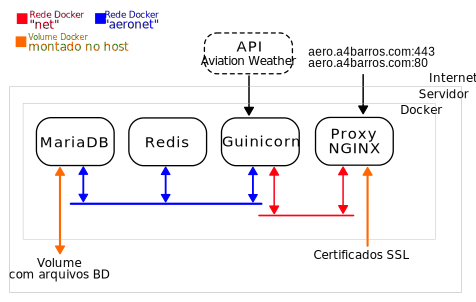
\includegraphics[width=\linewidth]{img/diagrama-arquitetura.png}
    \caption{Modelo de Arquitetura}
    \label{fig:arquitetura}
    \end{center}
\end{figure}

\section{Docker Network}
A porta 5000 do Gunicorn não estará disponível para todos os serviços. Por segurança, é usada a função de
"network". Observe no diagrama que a proxy NGINX compartilha com o Gunicorn a rede "net", para o NGINX,
o Gunicorn não pode ser acessado por \texttt{localhost:5000}, e sim por \texttt{http://aero:5000}, "aero"
sendo o nome do serviço no Docker Compose.


\section{Docker Secrets}

Para aumentar a segurança de acesso ao banco, é usada a funcionalidade "secrets". Nela, no Docker Compose,
você informa um arquivo de texto no host onde estará uma senha, uma senha por arquivo. No mesmo Compose,
você informa quais serviços têm acesso a cada senha. Caso o serviço de banco de dados, por exemplo, tenha
acesso a senha db-password.txt, será feito um bind do arquivo db-password.txt no host para o "/run/secret/db-password.txt"
no guest.
Tanto os bancos como o servidor Gunicorn usam este método para terem acesso às senhas dos bancos.

\section{Serviços}

\subsection{MariaDB}
Este banco de dados relacional guarda toda a informação mais ou menos fixa sobre os aeródromos,
conforme explicado no capítulo de modelo de dados.

\section{FastAPI}

O site foi construído com a framework FastAPI tanto para desenvolvimento quanto para produção, 
utilizando o servidor embutido do FastAPI, o Uvicorn.

Diferentemente do Flask, em que era necessário usar um servidor externo (o Gunicorn no caso 
deste projeto), o servidor do FastAPI (Uvicorn \cite{uvicorn}), com a configuração padrão, é 
suficiente para produção. Usando o comando \texttt{uvicorn server:app --host 0.0.0.0 --port 5000}, 
o servidor é iniciado em modo de produção.

\subsection{Proxy NGINX}
O NGINX faz o HTTPS funcionar, dá suporte ao HTTP/2 e ao cabeçalho HTTP keep-alive. Quando
utilizava o Gunicorn, ele só tinha suporte ao primeiro, e a documentação do Gunicorn não
recomendava que ele estivesse diretamente ligado à Internet \cite{nginx-gunicorn}. O Uvicorn,
no momento em que este texto foi escrito, não suporta HTTP/2, mas suporta o keep-alive. No
entanto, como tenho outros projetos na mesma máquina, utilizo subdomínios. Todos os subdomínios
resolvem para a mesmo IP/máquina via "A RECORD", mas na configuração
do NGINX, o bloco de servidor com o hostname aero.a4barros.com é redirecionado para o
endereço interno "http://aero:5000".

\section{Produção}
O site se encontra em produção no endereço https://aero.a4barros.com. Ele está hospedado em uma VPS
da Oracle Cloud Infrastructure com as seguintes características de hardware:

\begin{itemize}
    \item \textbf{CPU:} AMD EPYC 7551 (2 cores) @ 1.996GHz
    \item \textbf{RAM:} 1GB
    \item \textbf{Armazenamento:} 25GB
    \item \textbf{SO:} Ubuntu 22.04.4 LTS
\end{itemize}

\begin{figure}[ht]
    \begin{center}
    \includegraphics[width=400pt]{img/prod-idle.png}
    \caption{Uso do sistema em baixa demanda}
    \label{fig:prod-idle}
    \end{center}
\end{figure}

Mesmo com uma configuração bastante modesta, o sistema roda sete containers Docker, usando 
aproximadamente metade da memória primária (RAM) em idle.

\begin{figure}[ht]
    \begin{center}
    \includegraphics[width=400pt]{img/containers.png}
    \caption{Containers Docker em execução}
    \label{fig:containers}
    \end{center}
\end{figure}

\section{Diagrama de sequência}

\begin{figure}[ht]
    \begin{center}
    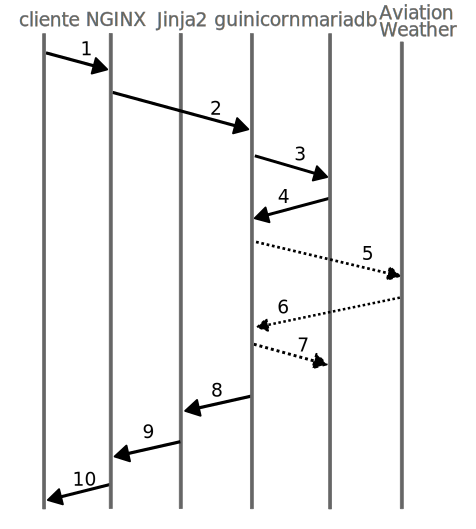
\includegraphics[width=0.5\linewidth]{img/diagrama-tempo.png}
    \caption{Diagrama de sequência}
    \label{fig:tempo}
    \end{center}
\end{figure}

\begin{enumerate}
\item O usuário realiza uma requisição para a rota raiz ou "/info/\{icao\}".
\item Um servidor NGINX funcionando como proxy realiza o limite de requisições por segundo
e bloqueia user-agents que aparentem ser robôs. Caso a requisição passe pelo filtro, é
realizado um proxy-pass para o servidor Gunicorn.
\item Para a rota raiz, é feito um SELECT no banco para pegar informações de todos os
aeroportos. Na rota "/info/\{icao\}", é feito um SELECT-WHERE para buscar apenas um aeroporto.
A ORM é usada para isto, portanto os comandos SQL não aparecem diretamente no código.
\item O banco de dados responde à requisição. Para a rota "/info/\{icao\}", é verificado 
se o METAR existente no banco é válido para aquela hora. Se for, o sistema vai para o passo 8;
se não, continua para o passo 5.
\item É feita uma requisição para a API do Aviation Weather pedindo o METAR para o 
aeroporto em questão. O sistema vai para o passo 3.
\item A API responde.
\item O METAR atualizado é gravado no banco.
\item O servidor envia as informações necessárias ao Jinja2 para a geração da página.
\item A página HTML é gerada.
\item O usuário recebe esta página.
\end{enumerate}

  \chapter{Front-end}

Como falado no capítulo da arquitetura, a página é gerada server-side, então o que 
é retornado para cada rota é um HTML já pronto. Acredito que, para o meu caso, é mais 
performático fazer assim do que usar páginas com Javascript que fazem requisição para uma API REST.

De todo modo, no final da execução de uma rota, um dicionário Python é gerado, algo que 
poderia ser facilmente convertido para um JSON usando a função \texttt{dumps()} da 
biblioteca \texttt{json} do próprio Python. No caso desta aplicação, este dicionário é 
enviado para o template usando a função \texttt{render\_template()} da biblioteca Jinja2, 
que recebe o nome da página HTML com o template e um número qualquer de \textit{kwargs} (argumentos nomeados) 
que podem ter qualquer tipo serializável, incluindo dicionários.

Perceba que não há problema de acoplamento fazendo deste modo, pois não há código HTML sendo 
escrito dentro do backend. Como já dito, o que é passado para o Jinja é algo equivalente a JSON.

Um página template é um arquivo HTML com \textit{placeholders} que serão substituídos pelos 
\textit{kwargs} de mesmo nome. O Jinja2 tem estruturas de repetição para que um código HTML 
possa ser repetido usando valores da lista. E, no caso de dicionários, é fácil acessar 
os valores. Neste projeto, para exibir a lista de frequência, o seguinte código é usado.

\lstinputlisting[label=cod:jinja-comm-old,title={Formatação Antiga},caption={Formatação Antiga},language=SQL]{code/jinja-comm-old.html}

Note que é possível fazer operações e formatações simples no Jinja2. Já que a frequência 
é armazenada no banco como um inteiro de ponto fixo (como dito no capítulo de modelo de dados), 
aqui eu poderia dividir o valor por mil e formatar com três casas decimais para que, caso 
uma frequência termine com zeros à direita, sempre tenhamos três dígitos decimais, que 
é o padrão para frequências de comunicação.

Porém, para não misturar a \textit{view} com o \textit{controller}, deixei este processamento 
de dados para uma função dentro do controlador.

\lstinputlisting[label=cod:jinja-comm,title={Formatação Atual},caption={Formatação Atual},language=SQL]{code/jinja-comm.html}

No código do projeto, na pasta 'templates', é possível ver todos os templates usados.

  % \chapter{Rotas do back-end}

\section{Rota raiz}

Página inicial, apresenta a lista de aeródromos para que o usuário escolha um. 
Internamente, por meio do ORM, é feita a seleção dos campos \texttt{AerodromeName},
\texttt{ICAO} e \texttt{City} e o resultado é posto em uma lista para cada um dos aeródromos e enviado
para a ferramenta de template criar a página.

Exemplo do resultado do banco:
\begin{verbatim}
[
    ('Presidente Juscelino Kubitschek', 'SBBR', 'Brasília'), 
    ('Tancredo Neves', 'SBCF', 'Belo Horizonte'), 
    ('Afonso Pena', 'SBCT', 'Curitiba'), 
    ('Pinto Martins', 'SBFZ', 'Fortaleza'), 
    ...
]
\end{verbatim}

\section{Rota: /info/\{ICAO\}}

Retorna informações de um aeródromo com o ICAO especificado na URL. São exibidos,
além da explicação do METAR atual:

\begin{itemize}
    \item Pista
        \begin {itemize}
        \item Cabeceiras
        \item Comprimento
        \item Largura.
        \end {itemize}
    \item Frequências do aeródromo (nem todos os items a seguir poderão estar disponíveis)
    \begin{itemize}
        \item Torre
        \item Solo
        \item Operações
        \item Rampa
        \item Tráfego
        \item ATIS
    \end{itemize}
    \item Frequências de navegação (nem todos os items a seguir poderão estar disponíveis)
    \begin{itemize}
        \item ILS
            \begin{itemize}
                \item Qual pista este ILS se refere
                \item Frequência
                \item Direção final de aproximação
                \item Identificador
            \end{itemize}
        \item VOR
            \begin{itemize}
                \item Frequência
                \item Identificador
            \end{itemize}
    \end{itemize}

\end{itemize}

\section{Rota: /history/\{ICAO\}}
Para um aeródromo retorna informações dos dez últimos METARs em três
gráficos com o eixo horizonal sendo o tempo.

\begin{itemize}
    \item Gráfico 1
    \begin{itemize}
        \item Temperature (graus Célsius)
        \item Ponto de orvalho (graus Célsius)
    \end{itemize}
    \item Gráfico 2
    \begin{itemize}
        \item Velocidade do vento (milhas náuticas por hora)
        \item Direção do vento (graus)
    \end{itemize}
    \item Gráfico 3
    \begin{itemize}
        \item Ajuste altímetro (hectopascal)
        \item Visibilidade (metro)
    \end{itemize}
\end{itemize}

\section{Rota: /taf/\{ICAO\}}
Retorna o próximo TAF válido para este aeródromo com a explicação de cada item.



  \chapter{Conclusão e Próximos Passos}

O desenvolvimento deste projeto busca juntar as funcionalidades comumente usadas na 
simulação de voo em uma plataforma acessível e amigável, buscando promover um 
maior nível de realismo na simulação de voo, aspecto desejado por quem leva
a simulação de voo "a sério".

A arquitetura implementada, utilizando Docker e Docker Compose, garante uma 
implementação modular, segura e, com o uso do Git, de fácil deploy caso seja 
necessário trocar o ISP no futuro. O uso de um banco de dados como
o MariaDB e da funcionalidade Docker Secrets para armazenar as senhas, proporciona um 
ambiente robusto para o projeto.
O uso de uma VPS modesta para hospedagem do projeto em produção demonstra a 
viabilidade do sistema em ambientes com recursos limitados.

... TODO
  \chapter{Apêndice A: Códigos Relevantes}

\lstinputlisting[label=cod:jinja-comm, title={Código da ORM}, caption={Código da ORM usando a biblioteca SQLAlchemy}, language=Python]{code/ORM.py}

\lstinputlisting[label=cod:metar, title={a}, caption={a}, language=Python]{code/METAR.py}

%\lstinputlisting[label=cod:taf, title={a}, caption={a}, language=Python]{code/TAF.py}

\lstinputlisting[label=cod:plot, title={a}, caption={a}, language=Python]{code/history.py}


  
  \arial
  \bibliographystyle{abnt-num} % \bibliographystyle{abnt-alf}
  \bibliography{main} 
\end{document}
